\chapter{Tesseract}
\label{appendix:tesseract}
This chapter shows the table outputting the results from the Tesseract training phase.

\section{Tesseract data results}
\label{appendix:tesseract_table}

\begin{table}[h!]
\centering
 \begin{tabular}{||c c c c||}
 \hline
 Experiment & Characters Identified & Characters Correct & Correct Percentage \\ [0.5ex]
 \hline\hline
 1 & 114 & 70  & 61.40 \\
 2 & 252 & 182 & 72.22 \\
 3 & 345 & 280 & 81.15 \\
 4 & 335 & 265 & 79.10 \\
 5 & 288 & 201 & 69.79 \\
 6 & 276 & 206 & 74.63 \\
 7 & 326 & 256 & 78.52 \\
 8 & 400 & 279 & 69.75 \\
 9 & 462 & 364 & 78.78 \\
 10 & 401 & 266 & 66.33 \\
 11 & 366 & 240 & 65.57 \\
 12 & 362 & 273 & 75.41 \\ [1ex]
 \hline
 \end{tabular}
 \caption{A table which shows the statistics from the correctly identified characters during the training process.}
\end{table}

\section{Training examples} \label{tesseract:training}
This section displays some of the training examples which are used in the image training process. Further examples can be found under the \texttt{tesseract\_training\_data/adaptive\_threshold\_training\_data}.
\begin{figure}[H]
  \centering
  \begin{subfigure}[h]{0.35\textwidth}
    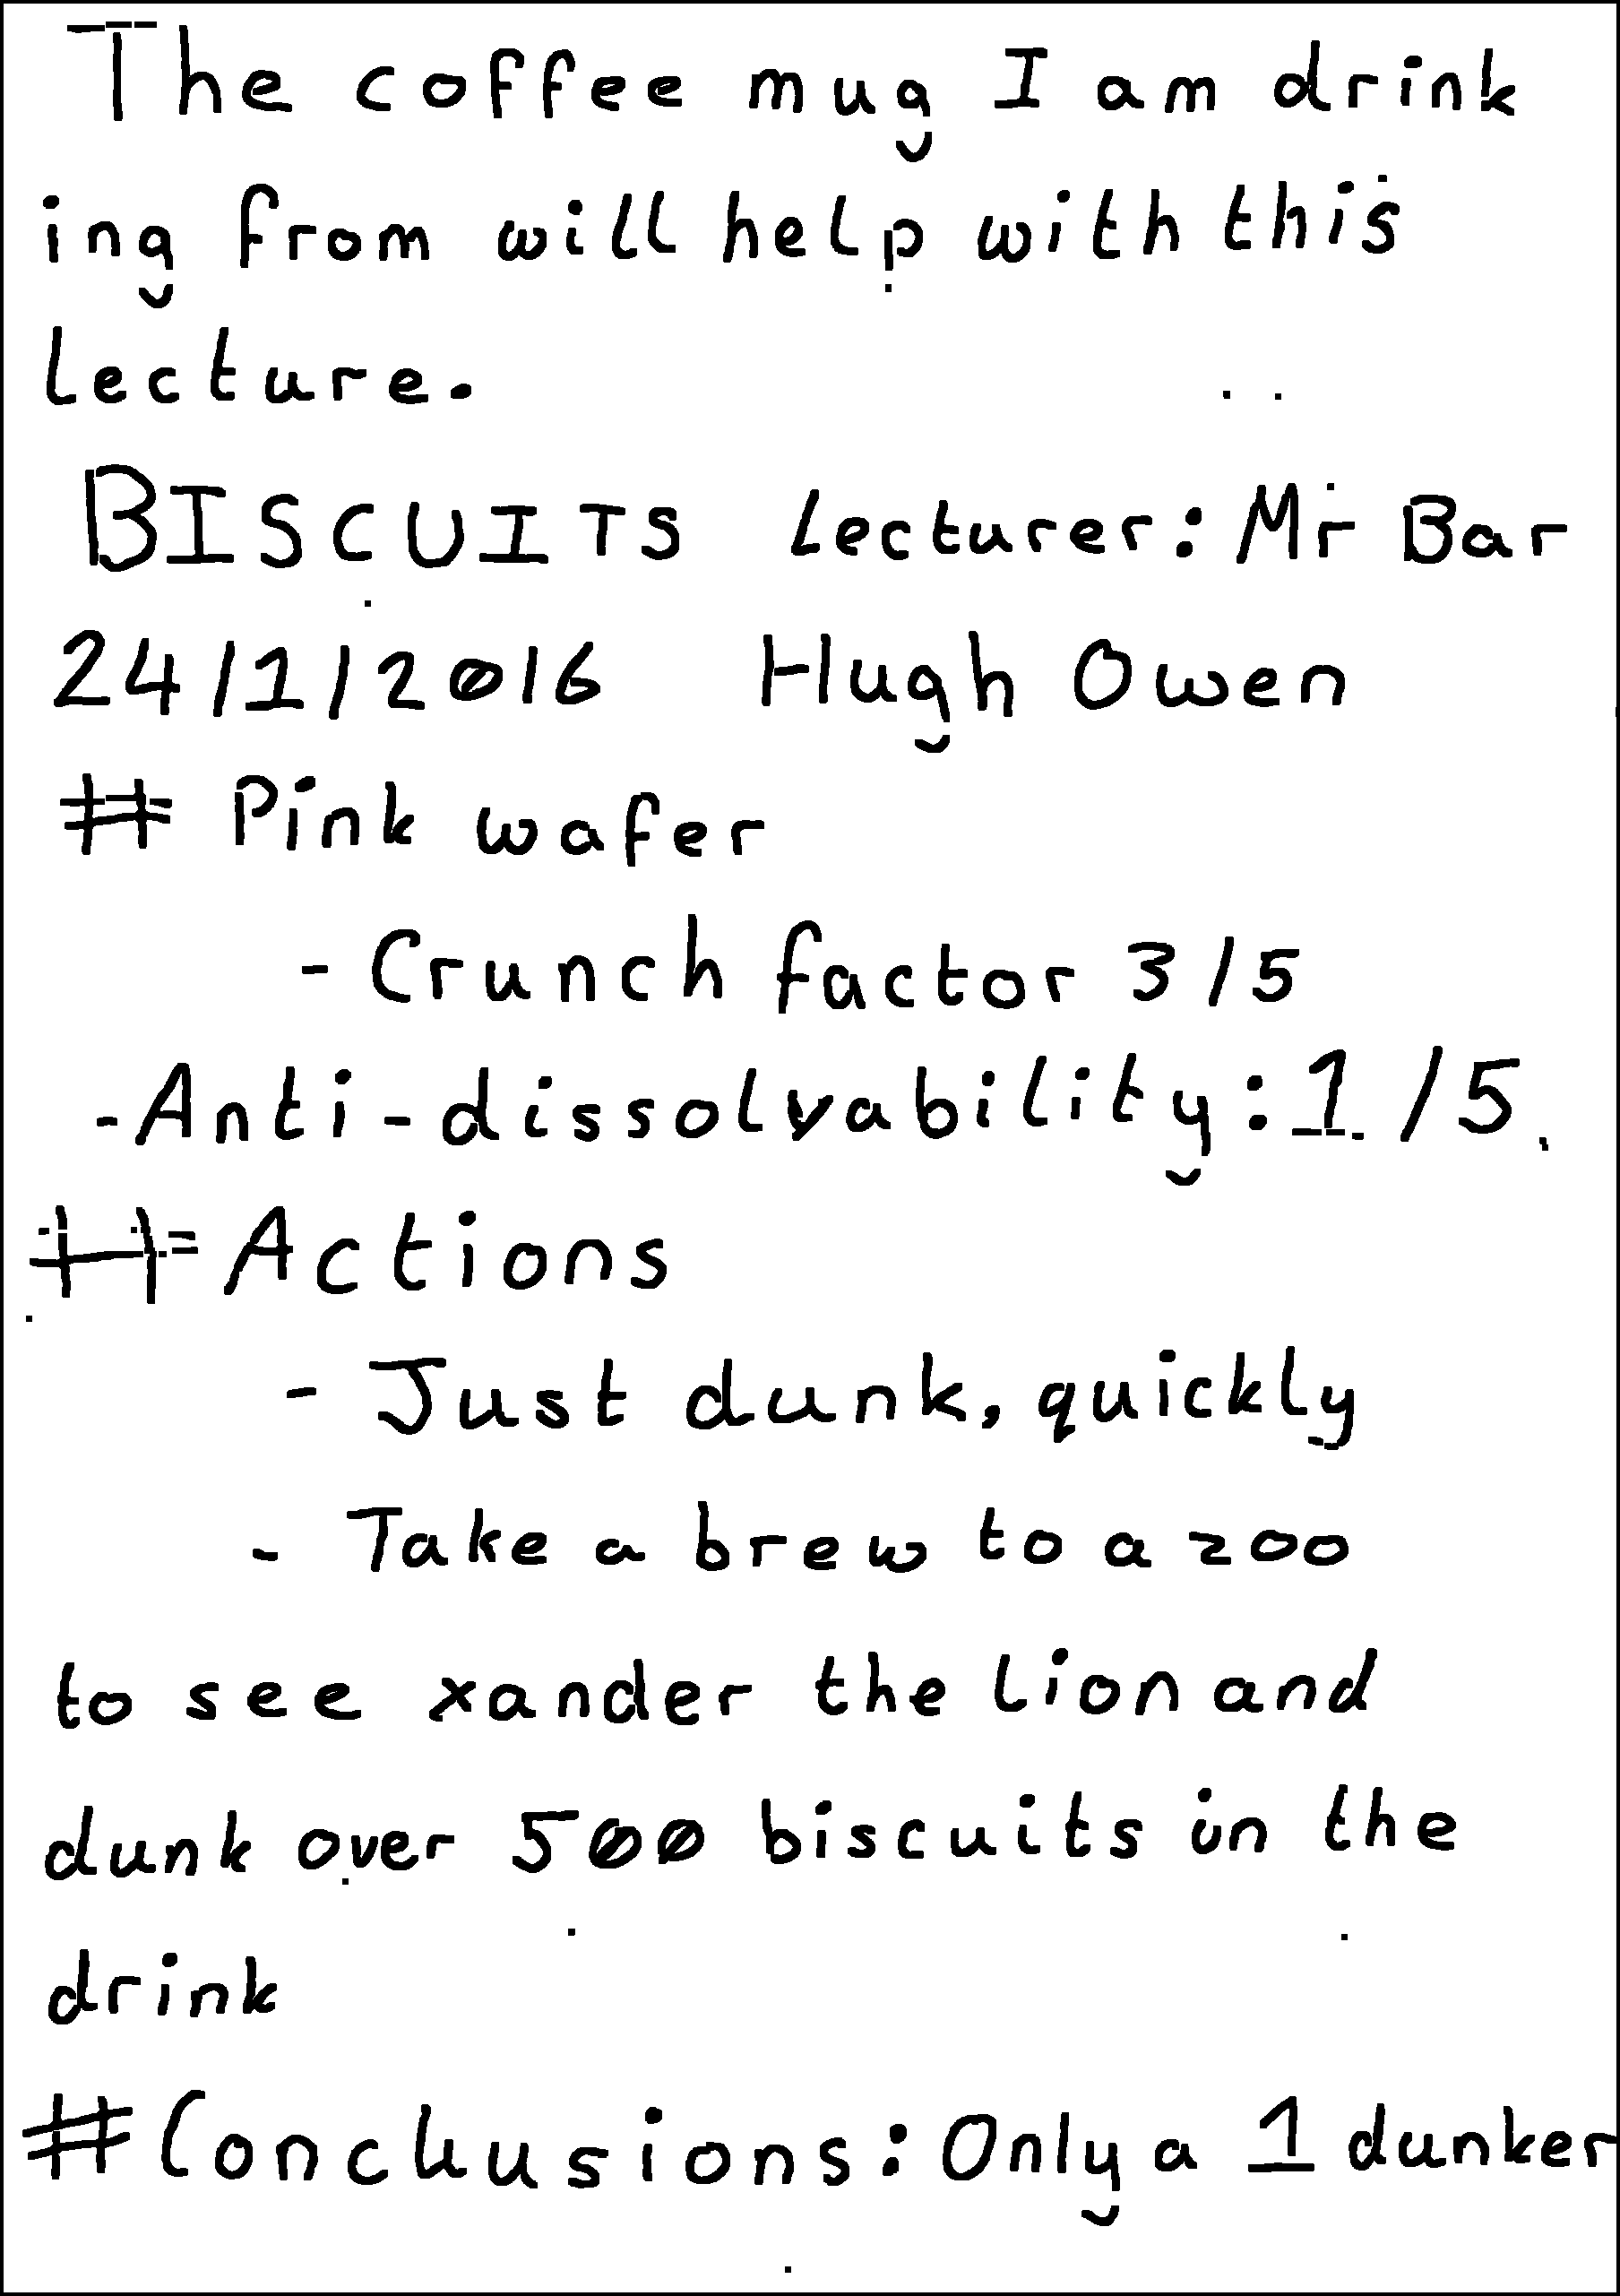
\includegraphics[scale=0.35]{images/training_data_1}
    \caption{}
    \label{fig:first_tesseract}
  \end{subfigure}

  \hspace{1em}

  \begin{subfigure}[h]{0.35\textwidth}
    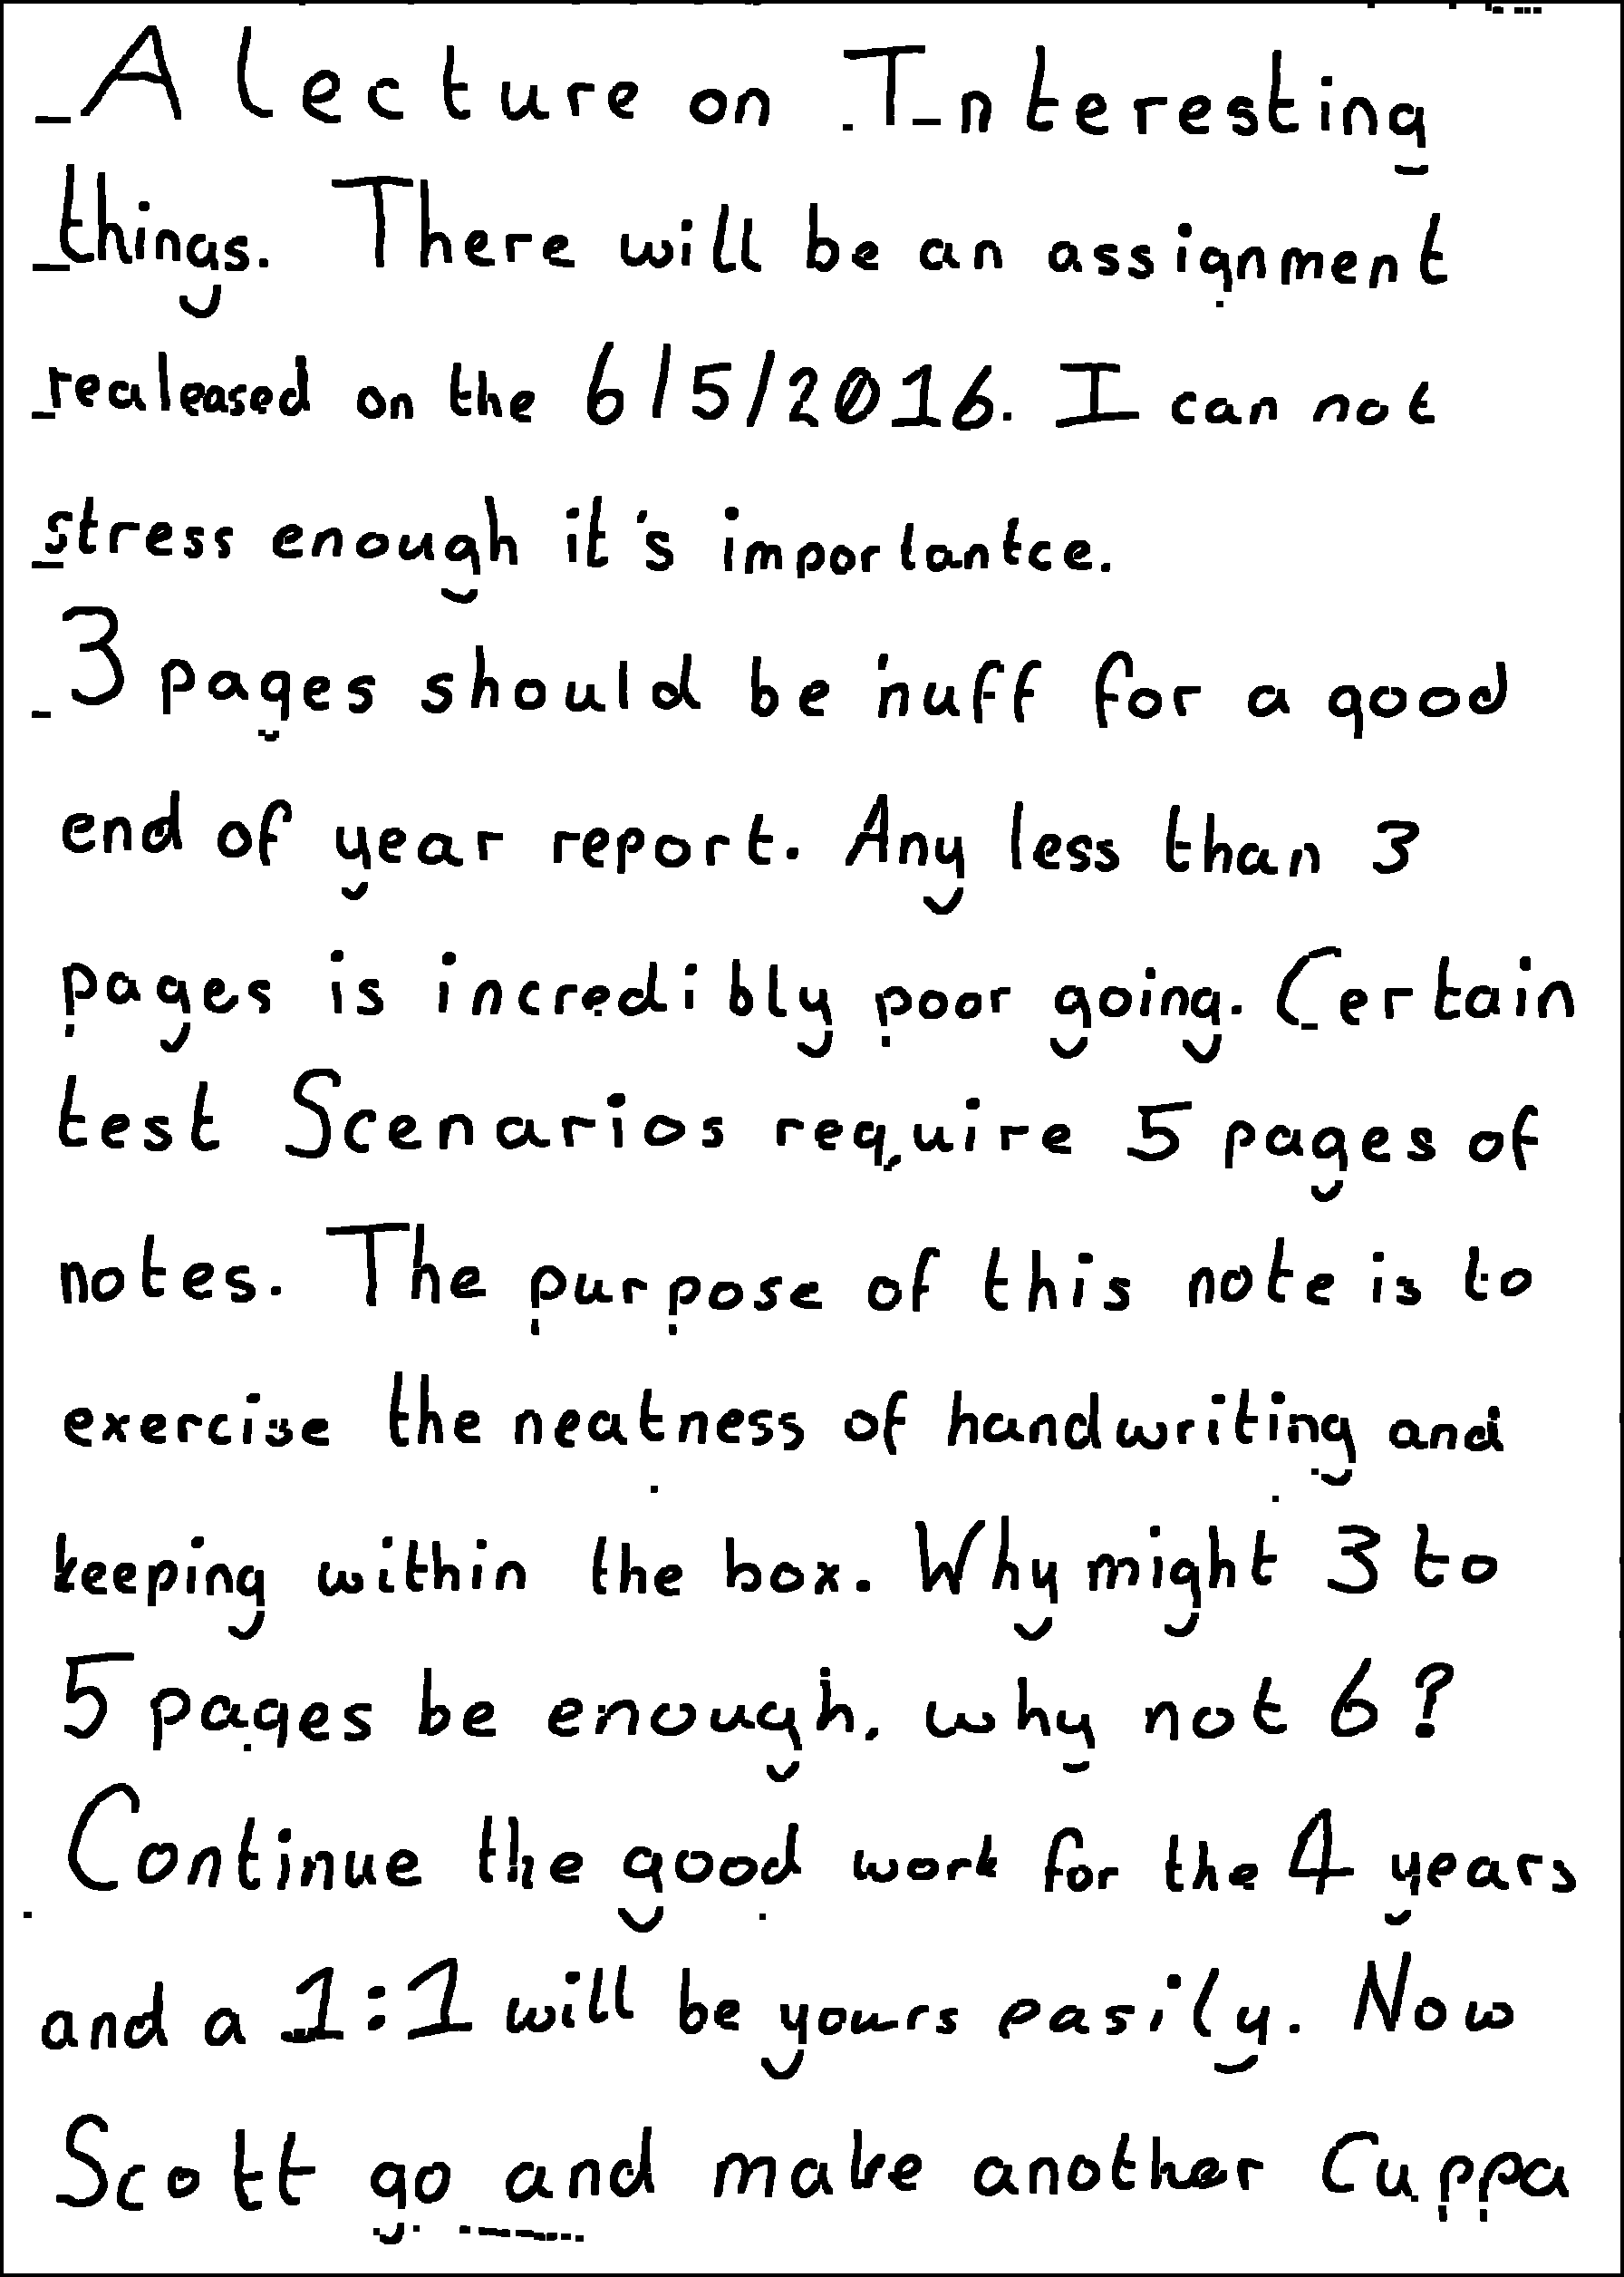
\includegraphics[scale=0.3]{images/training_data_2}
    \caption{}
    \label{fig:second_tesseract}
  \end{subfigure}

  \caption{An example of the binarised images used as part of the training data for the Tesseract engine.}
  \label{fig:tesseract_training data}

\end{figure}

\section{Pre-adaptive threshold results} \label{tesseract:spike_results}
\begin{table}[H]
\centering
\begin{tabular}{ ||p{3cm}||p{3cm}|p{3cm}|p{3cm}||  }
 \hline
 \multicolumn{4}{||c||}{Image pre-processing Spike work - Correctly identified characters} \\
 \hline
      Paper type & Greyscale & Original & Threshold\\
 \hline
  Blue-Lined & 18 &  36 & 75 \\
  Lined & 0 & 67 & 36   \\
  Plain & 0 & 0 & 63 \\
 \hline
\end{tabular}
\caption{Table showing the results of correctly identified characters in an image over different paper styles and different image processing steps.}
\label{table:pre-training}
\end{table}

\begin{table}[H]
\centering
\begin{tabular}{ ||p{3cm}||p{3cm}|p{3cm}|p{3cm}||  }
 \hline
 \multicolumn{4}{||c||}{Image pre-processing Spike work - Detected Characters} \\
 \hline
      Paper type & Greyscale & Original & Threshold\\
 \hline
  Blue-Lined &  85  & 119 &  157 \\
  Lined & 19 & 261 & 1186 \\
  Plain & 18 &  15 & 169 \\
 \hline
\end{tabular}
\caption{Table showing the results of the detected characters in an image over different paper styles and different image processing steps.}
\label{table:pre-training}
\end{table}
